\documentclass[11pt]{article}
\usepackage[letterpaper,margin=0.72in]{geometry}
\usepackage{amsmath,amssymb,amsthm,mathtools}
\usepackage{graphicx}
\usepackage[T1]{fontenc}
\usepackage{microtype}
\setlength{\parindent}{0pt}
\setlength{\parskip}{0.38em}
\setlength{\emergencystretch}{2em}
\newtheorem{theorem}{Theorem}
\newtheorem{lemma}{Lemma}
\newcommand{\C}{\mathbb C}
\newcommand{\Sp}{\mathcal S}
\newcommand{\F}{\mathcal F}
\newcommand{\HS}{\mathrm{HS}}
\newcommand{\IDA}{\mathrm{IDA}}
\newcommand{\supp}{\operatorname{supp}}
\title{Schatten rigidity for scaled Fock quantization\\
\large A sharp-range answer to the final problem in arXiv:2205.12345}
\author{Run \texttt{fa\_banach\_001} --- \texttt{agent\_lane\_03}}
\date{12 August 2026}

\begin{document}
\maketitle

\textbf{Status.} High-confidence candidate partial result, pending human
review.  It completely answers the Hilbert--Schmidt question in complex
dimension $n\ge2$, the trace-class question in every dimension, and more
generally every Schatten exponent $1\le p\le n$.  The range $p>n$ remains
open by this method.

\section*{The source question}
Let $\varphi\in C^2(\C^n)$ be real-valued with
$i\partial\bar\partial\varphi\simeq\omega_0$, and put
\[
 d\mu_t(z)=t^{-n}e^{-2\varphi(z/\sqrt t)}\,dv(z),\qquad
 \F_t^2(\varphi)=H(\C^n)\cap L^2(\mu_t).
\]
Writing $T_u^{(t)}=P^{(t)}M_u$, the source asks for the bounded $f$ such
that, for every bounded $g$,
\begin{equation}\label{Q}
 \|T_f^{(t)}T_g^{(t)}-T_{fg}^{(t)}\|_{S_p}\longrightarrow0
 \quad(t\downarrow0),
\end{equation}
especially for the Hilbert--Schmidt norm $p=2$.

\begin{center}
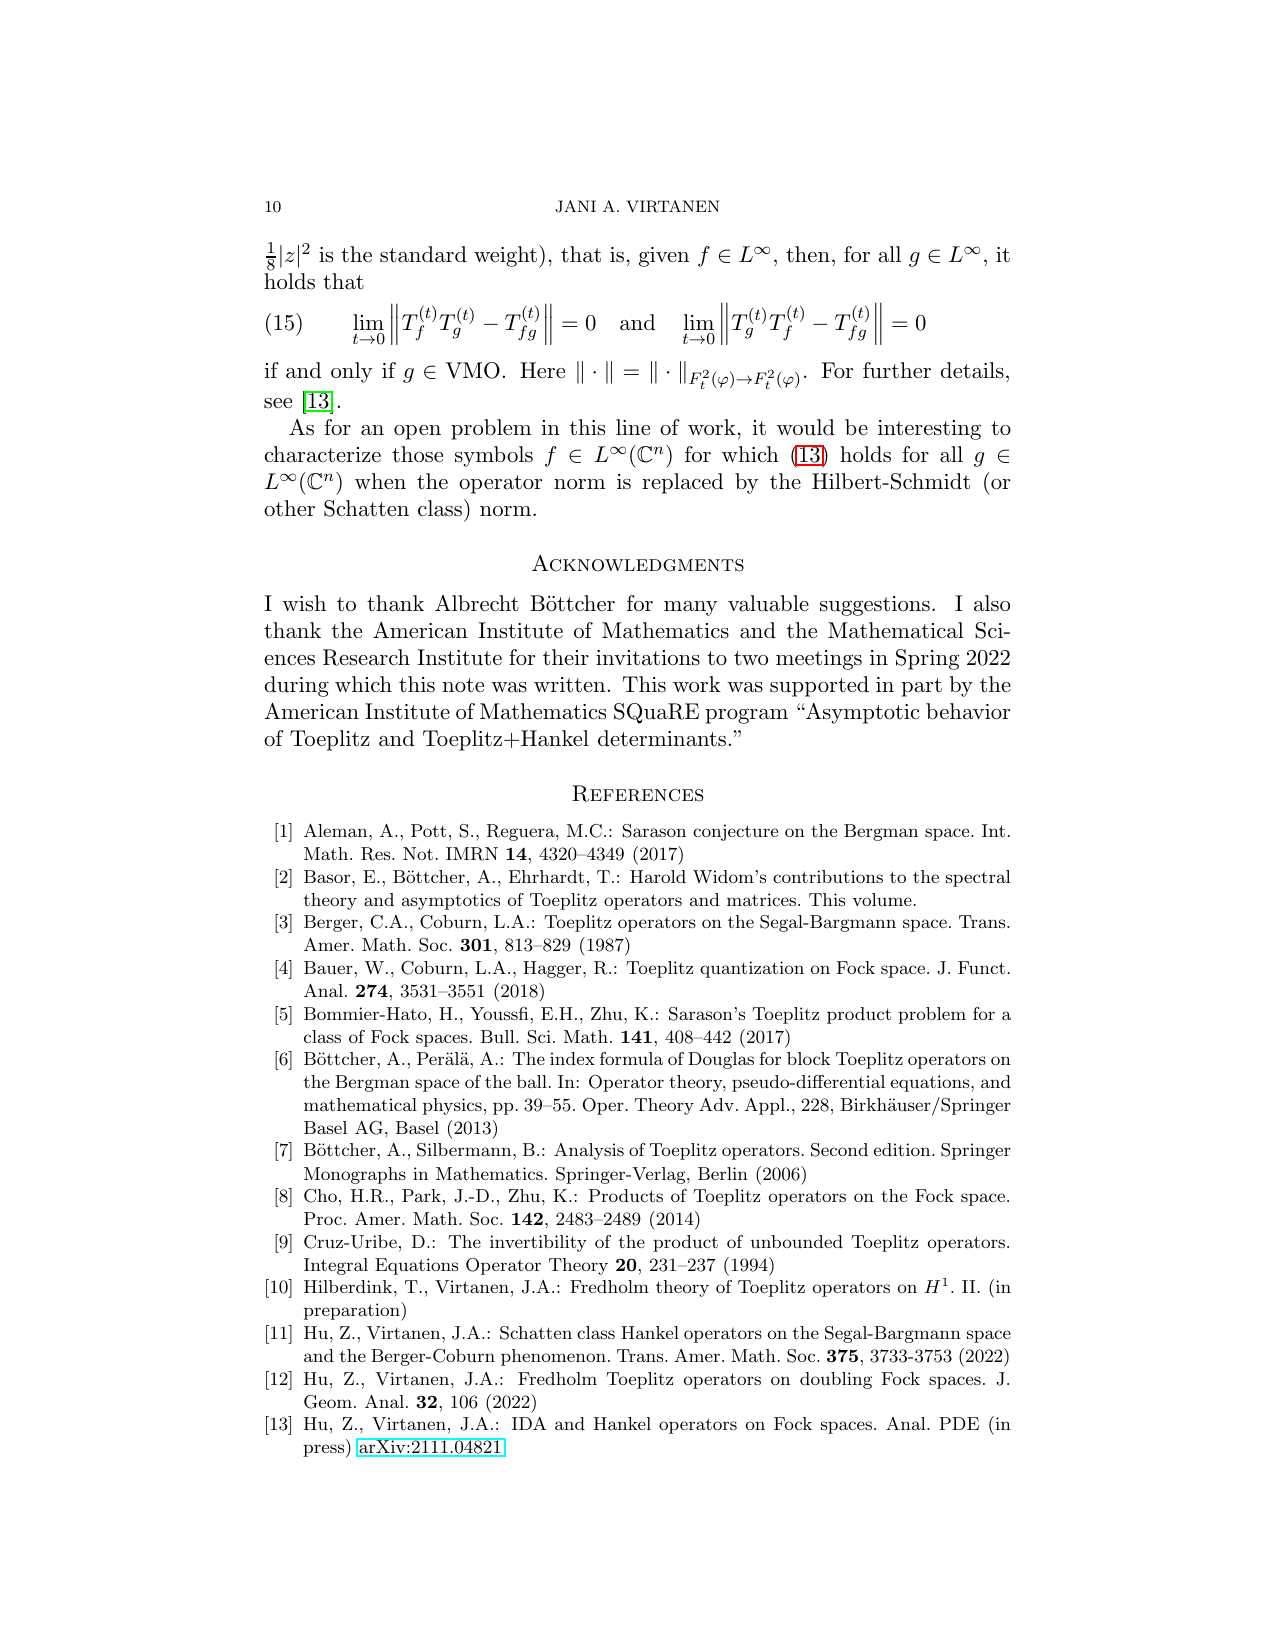
\includegraphics[width=0.92\textwidth,trim=70 510 70 165,clip]
 {figures/source_open_problem_page_10.png}
\end{center}
The exact page is bundled as
\texttt{source\_excerpt\_open\_problem\_page\_10.pdf}.

\begin{theorem}[sharp-range characterization]\label{thm:main}
Let $1\le p\le n$ and $f\in L^\infty(\C^n)$.  Then \eqref{Q} holds for
every $g\in L^\infty(\C^n)$ if and only if $f$ is constant almost
everywhere.  Consequently:
\begin{itemize}
 \item the Hilbert--Schmidt answer is exactly the constants when $n\ge2$;
 \item the trace-class answer is exactly the constants for every $n\ge1$.
\end{itemize}
\end{theorem}

\section*{Schatten/IDA input and its scaling}
For $u\in L^2_{\mathrm{loc}}(\C^n)$ define
\[
 G_r(u)(z)=\inf_{h\in H(B(z,r))}
 \left(\frac1{|B(z,r)|}\int_{B(z,r)}|u-h|^2\,dv\right)^{1/2}.
\]
Hu--Virtanen's Theorem 1.1 states, for every $q>0$,
\begin{equation}\label{HV}
 \|H_u\|_{S_q}\asymp \|G_1(u)\|_{L^q(\C^n)}.              \tag{HV}
\end{equation}
It applies here because $L^\infty$ lies in their symbol class $\Sp$.
The constants depend on $q,n,\varphi$, but not on $u$.

For $r=\sqrt t$, the unitary dilation
$U_t h(z)=h(rz)$ maps the scaled Fock space to the fixed space and
conjugates $H_u^{(t)}$ to $H_{u_r}$, where $u_r(z)=u(rz)$.  Moreover
\[
 G_1(u_r)(z)=G_r(u)(rz).
\]
Since $\C^n$ has real dimension $2n$, \eqref{HV} therefore gives the exact
scaling law, up to fixed comparison constants,
\begin{equation}\label{scale}
 \|H_u^{(t)}\|_{S_{2p}}
 \asymp r^{-n/p}\|G_r(u)\|_{L^{2p}(\C^n)}.               \tag{1}
\end{equation}

\section*{A rigidity lemma}
\begin{lemma}\label{lem:rigid}
Let $q\ge1$ and $u\in L^2_{\mathrm{loc}}(\C^n)$.  If
\[
 \|G_r(u)\|_{L^q}=o(r)\qquad(r\downarrow0),
\]
then $u$ agrees almost everywhere with an entire holomorphic function.
\end{lemma}

\emph{Proof.}
Choose $\eta\in C_c^\infty(B(0,1))$ with integral one and put
$\eta_r(x)=r^{-2n}\eta(x/r)$.  At each $x$, choose a holomorphic
near-minimizer $h_x$ in the definition of $G_r(u)(x)$.  Integration by
parts is legitimate because $\eta_r(x-\cdot)$ is compactly supported in
$B(x,r)$, and $\bar\partial h_x=0$.  Thus Cauchy--Schwarz gives, component
by component,
\begin{align*}
 |\bar\partial(u*\eta_r)(x)|
 &=\left|\int_{B(x,r)}(u(y)-h_x(y))
       \bar\partial_x\eta_r(x-y)\,dv(y)\right|\\
 &\le C r^{-1}G_r(u)(x).
\end{align*}
Indeed, the local $L^2$ error contributes $r^nG_r(u)(x)$, while
$\|\nabla\eta_r\|_2=O(r^{-n-1})$.  Hence
\[
 \|\bar\partial(u*\eta_r)\|_{L^q}
 \le Cr^{-1}\|G_r(u)\|_{L^q}\longrightarrow0.
\]
The mollifications converge to $u$ locally in distributions, so
$\bar\partial u=0$ distributionally.  Weyl's lemma for $\bar\partial$
finishes the proof. \qed

\section*{Proof of Theorem \ref{thm:main}}
The Fock product identity is
\[
 T_f^{(t)}T_g^{(t)}-T_{fg}^{(t)}
 =-(H_{\bar f}^{(t)})^*H_g^{(t)}.
\]
Use the universal quantifier in \eqref{Q} only once, with $g=\bar f$.
For every bounded operator $H$, membership of $H^*H$ in $S_p$ is
equivalent to membership of $H$ in $S_{2p}$, and
\[
 \|H^*H\|_{S_p}=\|H\|_{S_{2p}}^2.
\]
Consequently \eqref{Q} forces
$\|H_{\bar f}^{(t)}\|_{S_{2p}}\to0$.  Applying \eqref{scale} with
$u=\bar f$ yields
\begin{equation}\label{rate}
 \|G_r(\bar f)\|_{L^{2p}}=o(r^{n/p}).                    \tag{2}
\end{equation}
If $p\le n$, then $n/p\ge1$, and \eqref{rate} is in particular $o(r)$.
Lemma \ref{lem:rigid} says that $\bar f$ is entire.  It is bounded, hence
constant by Liouville's theorem, and so is $f$.

Conversely, if $f=c$ almost everywhere, then $T_f^{(t)}=cI$ and
$T_f^{(t)}T_g^{(t)}-T_{fg}^{(t)}=0$ for every $g$ and $t$. \qed

\section*{Proof intuition, sharpness, and remaining range}
The single adversarial choice $g=\bar f$ converts the semicommutator into a
positive Hankel square.  Schatten/IDA theory then translates small quantum
defect into the analytic-approximation rate $o(r^{n/p})$.  The geometric
threshold is exactly where that rate reaches first order: $p\le n$.
First-order decay kills $\bar\partial\bar f$ through mollification, leaving a
bounded entire function and therefore a constant.

For $p>n$, the forced exponent $n/p$ is below one, so the derivative estimate
need not vanish.  This is a genuine obstruction to this route: a nonconstant
smooth compactly supported $u$ has $G_r(u)=O(r)$ locally and hence passes the
necessary $g=\bar f$ test in that range.  The quantifier over all rough $g$
may still impose more, but no complete proof or counterexample was found.
Thus the packet does not claim the Hilbert--Schmidt answer in dimension one.

The result also separates the Schatten problem from the operator-norm answer:
nonconstant compactly supported smooth symbols lie in VMO, yet Theorem
\ref{thm:main} excludes them for Hilbert--Schmidt convergence when $n\ge2$.

\section*{References}
\begingroup\raggedright
\textbf{[1]} J. A. Virtanen,
\emph{On the product formula for Toeplitz and related operators},
arXiv:2205.12345, Section 5 and p.~10.

\textbf{[2]} Z. Hu and J. A. Virtanen,
\emph{Schatten class Hankel operators on the Segal--Bargmann space and the
Berger--Coburn phenomenon}, arXiv:2012.13768v2, Theorem 1.1.

\textbf{[3]} Z. Hu and J. A. Virtanen,
\emph{Corrigendum to ``Schatten class Hankel operators on the
Segal--Bargmann space and the Berger--Coburn phenomenon''},
arXiv:2012.13768v4.  The corrigendum changes Theorems 1.2 and 2.6, not the
Theorem 1.1 used above.
\par\endgroup

\end{document}
